
%%%%%%%%%%%%%%%%%%%%%%%%%%%%%%%%%%%%%%%%%%%%%%%%%%%%%%%%%%%%%%%%%%%%%%%%%%%
%
% Plantilla para un artculo en LaTeX en espaol.
%
%%%%%%%%%%%%%%%%%%%%%%%%%%%%%%%%%%%%%%%%%%%%%%%%%%%%%%%%%%%%%%%%%%%%%%%%%%%

\documentclass[11pt,oneside]{article}

% Esto es para poder escribir acentos directamente:
%\usepackage[latin1]{inputenc}
\usepackage[utf8]{inputenc}
\usepackage{makeidx}
\usepackage{multirow}
\usepackage{titlesec}
\usepackage{sectsty}
\usepackage{fncychap}

\usepackage{comment}

% Esto es para que el LaTeX sepa que el texto est en espaol:
\usepackage[spanish]{babel}
\usepackage[right=3cm,left=3cm,top=2.5cm,bottom=2.5cm,headsep=1cm,footskip=2cm]{geometry}
\usepackage{graphicx}
% Paquetes de la AMS:
\usepackage{amsmath, amsthm, amsfonts}

\usepackage{fancyhdr}
\pagestyle{fancy}
\lhead{
\chead{
\rhead{\bfseries Informe de Práctica }
%\lfoot{From: K. Grant}
%\cfoot{To: Dean A. Smith}
\rfoot{\thepage}
\renewcommand{\headrulewidth}{0.4pt}
\renewcommand{\footrulewidth}{0.4pt}
}}
\begin{document}
\setlength{\unitlength}{1 cm} %Especificar unidad de trabajo
\thispagestyle{empty}
\begin{picture}(0,1.5)
\put(0,0){
\includegraphics[width=2.7cm,height=2cm]{utfsm.jpg}}
\put(13,0){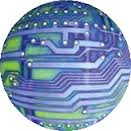
\includegraphics[width=2cm,height=2cm]{elo.jpg}}
\end{picture}
\\
\\
\begin{center}
\textbf{{\LARGE Universidad Técnica Federico Santa María}\\[0.5cm]
{\LARGE Departamento de Electrónica}}\\[4.25cm]
{\Large Informe de Práctica}\\[2.3cm]
{\LARGE \textbf{Centro Cient\'ifico Tecnol\'ogico de Valpara\'iso}}\\[3.5cm]
{\large Arturo Veras Olivos}\\[2cm]
Valparaiso - \today
\\
 {\large Versión 2.5}
\end{center}

%\newpage
%\tableofcontents
%\listoffigures % to produce list of figures
%\listoftables % to produce list of tables
\newpage
\section{Información General}

\subsection{Alumno}
\begin{tabular}{|l|l|}
\hline 
Nombre Completo: & Arturo Armando Veras Olivos \\ 
\hline 
Domicilio: & Garibaldi 205 - Cerro La Cruz, Valpara\'iso \\ 
\hline 
E-mail & a.veras@gmail.com \\ 
\hline 
Tel\'efono & +56 9 82413883 \\ 
\hline 
Rol USM: & 2521042-5 \\ 
\hline 
Carrera & Ingenier\'ia Civil Electr\'onica \\ 
\hline 
Curso: & Sexto año de la carrera \\ 
\hline 
Tipo de Pr\'actica & Profesional \\ 
\hline 
Fecha de inicio & 13/01/14 \\ 
\hline 
Fecha de t\'ermino & ??/03/14 \\ 
\hline 
Duraci\'on & 8 semanas \\ 
\hline 
\end{tabular} 
\subsection{Empresa}

\begin{tabular}{|l|l|}
\hline 
Nombre: & Centro Cient\'ifico Tecnologico de Valpara\'iso \\ 
\hline 
Direcci\'on: & Avenida España 1680, Valpara\'iso \\ 
\hline 
RUT:  & 81.668.700-4 \\ 
\hline 
Direcci\'on Web: & www.cctval.cl \\ 
\hline 
\end{tabular} 

\subsection{Supervisor}
\begin{tabular}{|l|l|}
\hline 
Nombre: & Claudio Torres \\ 
\hline 
Cargo: &   \\ 
\hline 
Oficio o profesi\'on:  & 81.668.700-4 \\ 
\hline 
Tel\'efono: & +56 (32) 2654418 \\ 
\hline 
E-mail: & ctorres@inf.utfsm.cl \\ 
\hline
\end{tabular} 
\newpage
\section{Resumen Ejecutivo}
\begin{comment}
El objetivo de esta sección es que una persona no especialista que lea este resumen conozca la actividad desarrollada por el alumno, los objetivos del trabajo realizado, la metodología y los recursos empleados, logros obtenidos, aporte realizado, etc.. Su extensión no debe superar una página.
\end{comment}
La práctica se desarrolla dentro de un grupo de investigación que se crea para construir un cluster de Raspberry Pi\footnote{Raspberry Pi es un ordenador de placa reducida o (placa única) (SBC) de bajo costo, desarrollado en Reino Unido por la Fundación Raspberry Pi, con el objetivo de estimular la enseñanza de ciencias de la computación en las escuelas.} y simultaneamente conectar cada Raspberry Pi a una tarjeta de video para aprovechar las capacidad de la GPU\footnote{La GPU, —acrónimo de «graphics processing unit», que significa «unidad de procesamiento gráfico»— es un procesador (como la CPU) dedicado al procesamiento de gráficos; su razón de ser es aligerar la carga de trabajo del procesador central y, por ello, está optimizada para el cálculo en coma flotante, predominante en las funciones 3D.} con el propósito de realizar HPC\footnote{HCP - acrónimo de «high performance computing» es una herramienta muy importante en el desarrollo de simulaciones computacionales a problemas complejos apoyandose en tecnologías computacionales como los clusters, supercomputadores o mediante el uso de la computación paralela.}.  Actualmente existen proyectos que han trabajado construyendo clusters\footnote{El término clúster - se aplica a los conjuntos o conglomerados de computadoras construidos mediante la utilización de hardwares comunes y que se comportan como si fuesen una única computadora.} utilizando la Raspberry Pi de 8, 32, y 42 nodos oteniendo buenos resultados. 

La idea surge a partir de tener un dispositivo para HPC que sea de bajo costo utilizando computadoras de bajo costo como la Raspberry Pi y tarjetas de video. La idea está orientada a investigadores, docentes, científicos o cualquier tipo de proyecto que necesiten realizar cálculos de mucha complejidad y que no dispongan de grandes recursos económicos para ello. En síntesis el producto final corresponde a un cluster de mini computadoras, cada uno con su respectiva GPU, el cual será capaz de correr programas para computación de alto rendimiento evitando usar costosa supercomputadoras y poder aprovechar cualquier computadora de escritorio que pueda conectarse al clúster. 

El trabajo consiste en investigar la forma de conectar un mini computado Raspberry Pi a una tarjeta de video NVIDIA GT640, analizar la fáctibilidad de la conexión entre ambos dispositivos y finalmente, si es efectiva la conexión, realizar la implementación de modelo de prueba que pueda ser presentado para un posterior desarrollo como producto final. De no ser factible,  se realizará una documentación de las alternativas analizadas y del porqué no es posible dicha conexión. 

\section{Actividad del Lugar de Trabajo}
\begin{comment}
Describa la misión de la empresa, los procesos o funciones que se realizan en su lugar de trabajo, los proyectos que se están desarrollando, los problemas que se están enfrentando, etc.
\end{comment}
\section{Organigrama de la Empresa}
\begin{comment}
Incluir un diagrama con la organización interna de la empresa, que permita localizar el área o sección donde realizó la práctica.
\end{comment}

\section{Preparaci\'on de la pr\'actica}
\begin{comment}
Indique los tópicos, entre los que ha cursado hasta el momento, más requeridos durante el desarrollo de la práctica, y los que le hicieron falta para un mejor desempeño.
\end{comment}
\section{Sugerencia de Proyecto Innovador}
\begin{comment}
En no más de una página, sugiera usted formas de optimizar las tareas que se realizan, o un proyecto de modernización, modificación, expansión, desarrollo o investigación posible para la empresa.
\end{comment}
\end{document}
